\section{Introduction}
\label{sec:intro}

Federated learning (FL) enables distributed clients to train a shared model while keeping raw examples local~\cite{pmlr-v54-mcmahan17a}. Non-IID data and unequal local computation can cause client drift and objective inconsistency~\cite{li2020federated,10.5555/3495724.3496362}, while limited memory, processing capacity, and bandwidth restrict participation~\cite{MAL-083,9084352}. These challenges interact in hierarchical systems, where learning must accommodate distributed data and resources.

Hierarchical FL (HierFL) organizes communication through edge aggregators~\cite{9148862,9488756,rana2022hierarchical}, while split learning (SL) distributes network computation across devices and servers~\cite{GUPTA20181,vepakomma2019split}. SplitFed and HierFL methods combine partitioned execution with federated synchronization~\cite{thapa2022splitfed,quan2023hiersfl,10980018}. Conventional split execution exchanges intermediate activations and backward gradients, coupling successive segments during optimization. H-SFP uses a statistical interface: class means and diagonal standard deviations define Gaussian summaries from which upper tiers synthesize training features, enabling training without cross-tier backpropagation~\cite{tran2026h}.

The effectiveness of this interface depends on the structure retained by each class summary. A class can contain multiple feature clusters within one client or across client subpopulations (Fig.~\ref{fig:illustration}(a,b)). Collapsing separated clusters into one Gaussian can allocate density to regions between them, even when class means and coordinate-wise variances are preserved (Fig.~\ref{fig:illustration}(c)). A full covariance captures correlations at quadratic storage cost, but a single Gaussian remains unimodal. Multiple diagonal components offer several centers while keeping per-component moment storage linear in feature dimension.

\begin{figure*}[t]
\centering
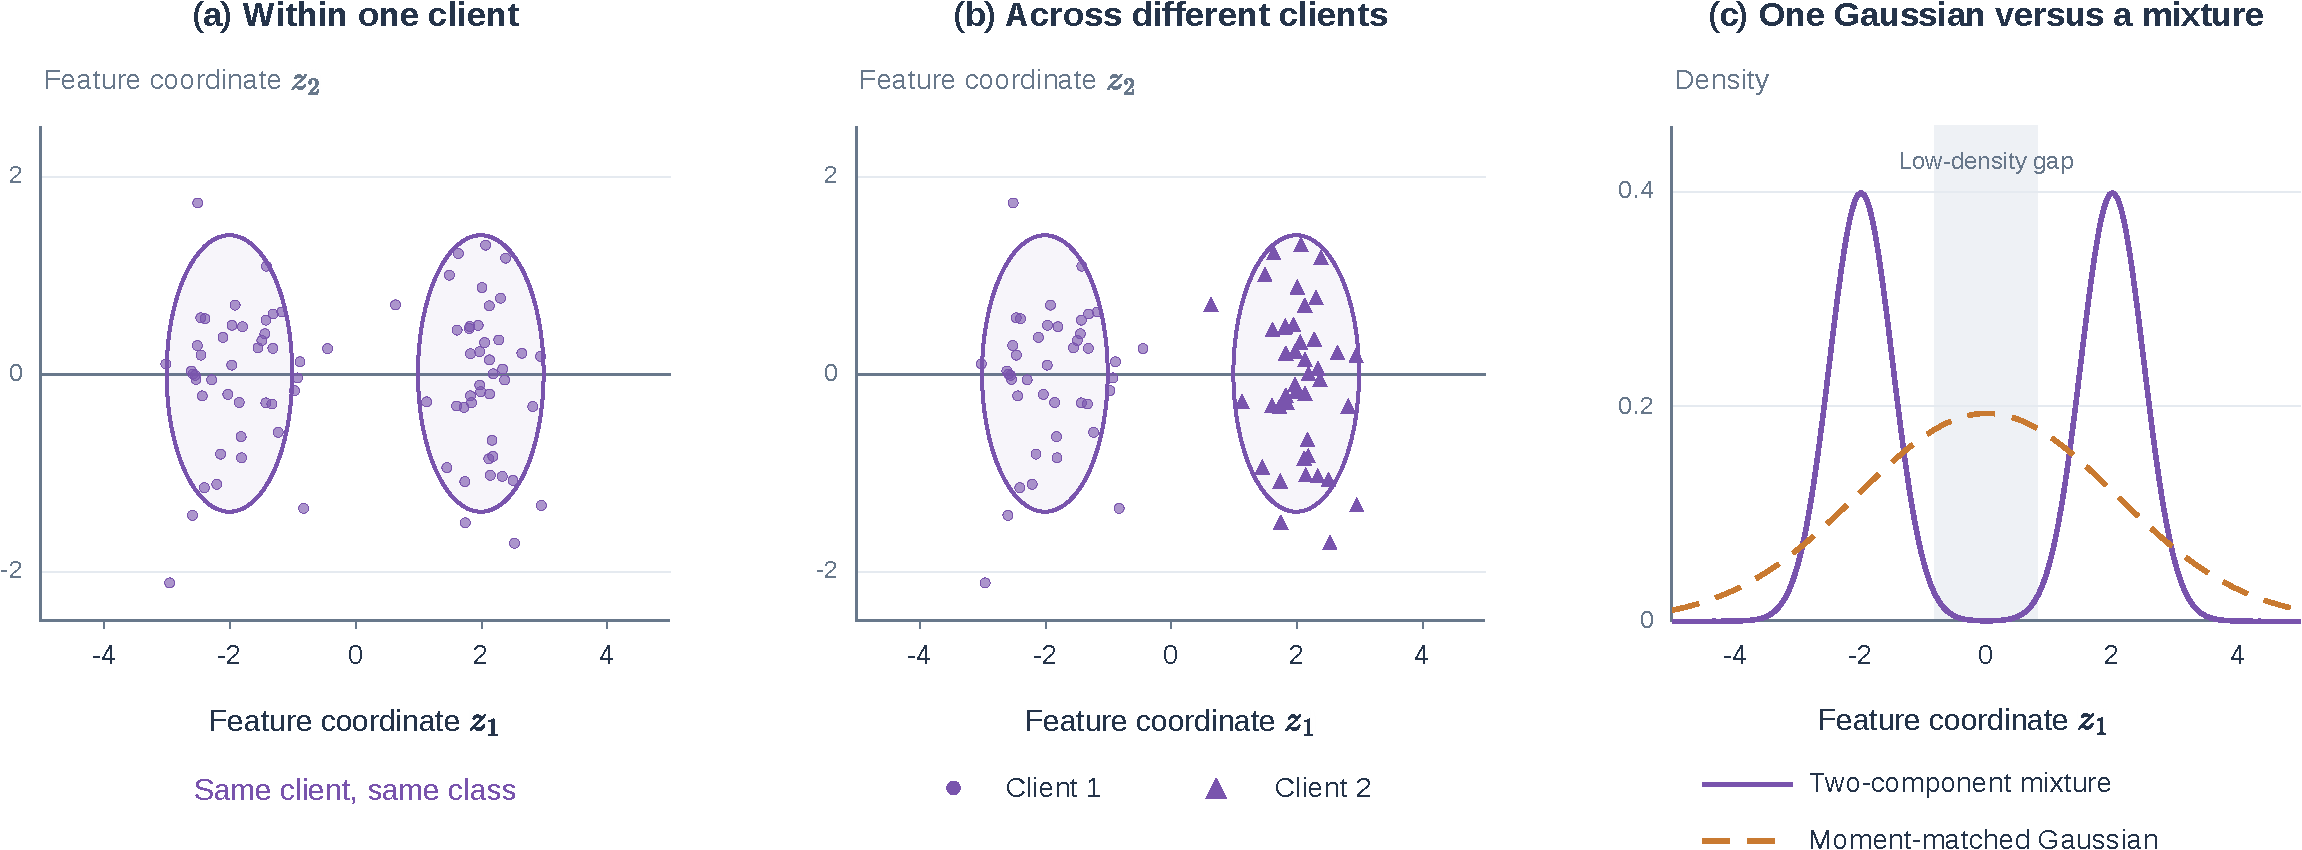
\includegraphics[width=\linewidth]{figures/misfp_multimodality.pdf}
\caption{Illustration of within-class multimodality: (a) modes within one client and (b) modes contributed by different clients. (c) First-coordinate marginal densities of a two-component mixture and its moment-matched single Gaussian. In this example, moment matching preserves the class mean and coordinate-wise variances but allocates more density between the modes.}
\label{fig:illustration}
\end{figure*}

Prototype learning, distillation, and generation establish the value of transferring compact class information and synthetic features~\cite{tan2022fedproto,lin2020ensemble,zhu2021data}. CCVR and FedImpro reconstruct feature distributions for classifier calibration or high-level training~\cite{luo2021ccvr,tang2024fedimpro}. FedPFT transfers parametric distributions from frozen foundation-model embeddings for one-shot classifier training~\cite{beitollahi2025fedpft}, while FedGMKD uses Gaussian mixtures to derive prototype features and soft predictions~\cite{zhang2024fedgmkd}. These provide foundations for distribution-based learning. Hierarchical split training additionally requires repeated transformation and compression as successive, spatially distributed model parts.

Three considerations govern this process. First, local class support constrains which components can be estimated reliably, while communication capacity limits their retention. Second, the nonlinear edge segment changes the feature distribution, requiring statistics to be re-estimated in its output space. Third, independently updated model segments can produce apparent separation through coordinate mismatch as well as population variation. Component allocation must therefore be considered jointly with support weighting, boundary transformation, coordinate compatibility, and packet cost.

We introduce \method{}, a hierarchical split-training framework that communicates support-weighted mixtures of diagonal Gaussians. Clients construct mixtures using fixed component requests or a validation-based selection heuristic. Receiving tiers retain same-class components and use deterministic greedy merges when compression is required. The edge trains from mixture samples and re-estimates output-space statistics before transmission to the cloud. Component caps and optional serialized-byte budgets control retention separately at the client--edge and edge--cloud boundaries. Gradients remain within each tier, while total communication includes periodic model synchronization.
The main contributions are:
\begin{enumerate}
    \item A support-weighted mixture interface for representing multiple class-conditional components and generating upper-tier training features in a hierarchical split model.

    \item A construction and compression procedure combining fixed or validation-selected local component counts, nonlinear-boundary re-estimation, and deterministic same-class merging under component caps and optional boundary-specific byte budgets.

    \item An analysis establishing exact mass and diagonal-moment preservation, bounding the transport discrepancy introduced by an individual merge, and characterizing packet costs, computational complexity, and fixed-predictor loss discrepancies under explicit assumptions.

    \item An evaluation combining classification and segmentation benchmarks with ablations of component retention, packet budgets, representation fidelity, encoder compatibility, and communication and resource costs.
\end{enumerate}